% For some reason only opens in Skim but can then export to working PDF...

%-------------------------------------------------------------------------------
% Preamble
%-------------------------------------------------------------------------------

\documentclass[a4paper, 12pt]{article}
\usepackage{ms}            % load the template
\usepackage[osf]{mathpazo} % palatino
\usepackage[round]{natbib} % author-year citations
%\usepackage[superscript,biblabel]{cite} % for superscript citations
\usepackage{graphicx}
\usepackage{subcaption}
\usepackage{parskip} 
\usepackage{amsmath}
\usepackage{longtable}
\usepackage{pdflscape}

\pagenumbering{arabic}  
\linespread{1.66}

%-------------------------------------------------------------------------------
% Title page information
%-------------------------------------------------------------------------------

\title{Comparative analyses of bite-force among lepidosaurs}
\author{}
\date{}
\affiliation{}

% remove these blank entries and uncomment the ones below when not double blinding

%\author{
 % Justin E Isip$^{1,2*}$,
  %Natalie Cooper$^{1}$, 
  %Marc EH Jones$^{3}$, 
%}
%\date{}
%\affiliation{\noindent{\footnotesize
 % $^1$Department of Life Sciences, Natural History Museum, Cromwell Road, London, SW7 5BD, UK.\\
  %$^2$Department of Life Sciences (Silwood Park), Imperial College London, Ascot, UK.\\ 
  %$^3$Research Department of Cell and Developmental Biology, Anatomy Building, University College London, Gower Street, London, WCIE 6BT, UK.\\
  %$*$Email address: XXX
%}}

\vfill

\runninghead{Bite-force in lepidosaurs}
%\keywords{}
%}

%-------------------------------------------------------------------------------
% Begin document
%-------------------------------------------------------------------------------
\begin{document}
\modulolinenumbers[1]   % Line numbering on every line

\mstitlepage

\parindent = 1.5em
\addtolength{\parskip}{.9em}

\raggedright

%-------------------------------------------------------------------------------
% Author info page to separate off for double blind review
%-------------------------------------------------------------------------------

%\section{Author contributions} 
%All authors conceived the ideas and designed methodology; JEI collected the data; JEI and NC analysed the data; all %authors contributed to writing drafts and gave final approval for publication.

%\section{Acknowledgments}
%We thank previous authors for sharing their data. We thank  St\'ephane J. Montuelle and Geoff While for correspondence.

%\section{Data accessibility}\label{data-code-and-materials}
%Data are available from the NHM Data Portal at https://doi.org/10.5519/dkrhpxjh. 
%R code is available from GitHub (https://github.com/nhcooper123/lepidosaur-biteforce; Zenodo DOI: To be added on acceptance).

%\section{Funding}
%This work was not supported by any grant funding.

%\newpage

%-------------------------------------------------------------------------------
% Abstract
%-------------------------------------------------------------------------------

\section{Abstract}

\begin{enumerate}

\item Bite-force is a performance trait related to many aspects of an animal’s ecology and life history. Bite-force tends to increase with head and body size, as larger individuals will have greater muscle cross-sectional area and in turn greater bite-force. Previous work has suggested that aspects of species ecology may influence bite-force beyond simple scaling relationships.

\item The majority of bite-force studies have focused on lepidosaurs (lizards, amphisbaenians and tuatara) because of their diversity and experimental tractability. However these studies usually only examine a single species or compare several closely related species, rather than taking a clade-wide approach.

\item Here we investigated the relationships between body size, head dimensions and bite-force performance across 161 species of lepidosaur, using existing in vivo bite-force data from the literature and phylogenetic generalised least squares (PGLS) models. We then investigated how these relationships varied with respect to higher taxonomic groupings, diet, tooth attachment, and substrate use (e.g. fossorial, saxicolous, arboreal). 

\item We found that bite-force is strongly related to body size across lepidosaurs, and that species with the widest, longest and/or tallest heads have the greatest bite-forces. Ecological factors such as diet and substrate use show little explanatory power for bite-force, though fossorial species appear to bite more forcefully than expected given their body size and head dimensions, and in some models carnivores bite more forcefully than omnivores given their body size.

\item The weak relationships we report among ecology and body size/bite-force relationships may be the result of data limitation. Our results highlight that available data on bite-force in lepidosaurs is patchy, and skewed towards certain groups. Our dataset included only 2.31\% of 7,107 extant lepidosaur species, and we had no data for many families. Many species remain unstudied and further species have been studied but the raw data required for meta-analysis is unavailable. Future studies should aim to provide their raw individual bite-force and morphological measurement data to facilitate the comparisons necessary for understanding border evolutionary patterns. 

\end{enumerate}

\textbf{Keywords: biteforce, diet, head shape, acrodonty, scaling}

%-------------------------------------------------------------------------------
% Main text
%-------------------------------------------------------------------------------

\section{Introduction}\label{main}
Bite-force is an important performance trait with close ties to ecology and life history \citep{herrel1999morphology,anderson2008bite,erickson2014comparative,lappin2014reliable,husak2009fitness}. 
It has been studied to better understand the relationship between form and function \citep{erickson2014comparative,schaerlaeken2012built}, ontogenetic scaling \citep{erickson2003ontogeny,herrel2006ecological,becerra2011bite,marshall2012ontogenetic,jones2009bite,lappin2017bite}, differences between captive and wild animals \citep{erickson2004comparison}, urbanisation \citep[e.g.][]{baxter2019street}, sex related differences \citep{herrel1999sexual,lappin2006biteB,jones2020reproductive, lappin2006gapingA} and to test biomechanical models \citep[e.g.][]{groning2013importance,montuelle2015vivo,sellers2017ontogeny}.
Bite force has also been examined with respect to feeding capacity and variation in diet \citep{huber2005analysis,santana2010mechanics,marshall2012ontogenetic,erickson2003ontogeny}.
Greater bite-force may reduce prey handling times and increase dietary breadth \citep{herrel1999morphology,herrel2004omnivory,verwaijen2002relationships,van2006seed,broeckhoven2014under,taverne2020proximate}. 
In some species of lizard, greater bite-force is also an effective predictor of success in staged dominance interactions or territory contests \citep{lailvaux2004performance,lappin2005weapon}, the outcome of male-male combat \citep{husak2006bite,huyghe2005morphology,lailvaux2004performance}, and reproductive success in natural populations \citep{husak2006bite,husak2009fitness,lappin2005weapon}.

Typically in vivo bite-force data are collected using a calibrated instrument with adjustable bite plates that can be placed in the animal's mouth \citep[e.g.][]{herrel1999sexual,anderson2008bite}. 
Generally, between three to five defensive bites are recorded for each animal, with a rest period of a minute or more between each bite \citep[e.g.][]{herrel1999morphology,lappin2006biteB} and the greatest bite-force, maximum performance, is used for comparisons among individuals \citep{hertz1988time}. 
Bite-force varies depending on the part of the jaw used and is greater at the posterior of the jaws nearer the insertion of the muscles \citep[e.g.][]{groning2013importance}. 
Therefore bite-force data may be standardised for bite location using the outlever of the jaw \citep{lappin2014reliable}, or more commonly, bites are restricted to a particular part of the jaw such as the anterior tips \citep[e.g.][]{herrel1999morphology} or a specific tooth \citep[e.g.][]{erickson2003ontogeny}. 

Voluntary \textit{in vivo} bite-force has been successfully measured in a wide range of taxa, including sharks, frogs, crocodylians, rodents, and bats \citep{dessem1992jaw,herrel1999morphology,huber2005analysis,santana2010mechanics,erickson2014comparative,becerra2013biting,lappin2014reliable,lappin2017bite}. 
Most studies, however, have focused on lepidosaurs (lizards and tuatara) due to their experimental tractability and the apparent importance of bite-force to many aspects of their ecology and life history. 
Clade-wide variation in diet \citep[e.g.][]{cooper2002distribution,meiri2018traits}, food processing \citep[e.g.][]{mcbrayer2002prey,vitt2003history}, muscle anatomy \citep[e.g.][]{haas1973muscles,daza2011jaw}, and skull shape \citep[e.g.][]{metzger2005correlations} have been investigated across Lepidosauria. 
However, similar large scale analyses of variation in bite-force and its relationship to key traits such as diet, size, and substrate are lacking. Most studies instead focus on a single species \citep[e.g.][]{lappin2006gapingA,jones2020reproductive} or a set of closely related species \citep[e.g.][]{d2018increasing,taverne2020proximate}. 
This restricts our ability to identify meaningful general patterns with respect to key traits (such as size, diet, and substrate or habit) that could inform predictions for taxa that cannot be measured directly due to size, rarity, or extinction. 
A clade-wide comparative approach is required to understand how and why bite-force varies among species and to test related hypotheses.
In this study we use a clade-wide comparative approach to investigate variation in bite-force within Lepidosauria in relation to species' morphological and ecological traits. 

Several morphological traits are predicted to be related to variation in bite-force across species. Bite-force tends to show positive allometric scaling with morphological traits, as larger individuals will have more muscle mass and presumably a greater bite-force \citep{aguirre2002ecomorphological,lailvaux2004performance,MEASEY2009217,herrel2004omnivory,vanhooydonck2005does}.
Independent of differences in overall body size, head dimensions are also strongly associated with bite-force performance \citep{jones2020reproductive,kaliontzopoulou2012relationships}, as animals with larger or wider heads are assumed to accommodate more jaw musculature which results in a greater bite-force \citep{herrel1999morphology,huyghe2005morphology,lappin2006biteB}.
Lepidosaurs also exhibit variation in how their teeth are attached to the jaw bone: pleurodonty, which involves teeth attached to the side of the jaw bone, or acrodonty, which involves teeth attached to the crest of the jaw bone \citep{smith1958evolutionary}.
Acrodonty has long been associated with greater anchorage and greater loading \citep[e.g][]{smith1958evolutionary,jones2008skull,fraser1983ecology,whiteside1986head} and recent analyses appear to support that association \citep{jenkins2020bite}.

Ecological variation may also contribute to differences in bite-force between species. Among carnivores bite force is related to dietary breadth, prey size, and prey handling times \citep{verwaijen2002relationships,herrel2006ecological}.
Herbivorous species are often considered to have greater bite-forces than carnivores and omnivores due the forces required to process fibrous plant material \citep{cooper2002distribution,herrel1999morphology,metzger2005correlations,herrel2004omnivory,Herrel2008}.
Species that feed upon hard-shelled prey (e.g. shelled molluscs, crabs, corals etc.) such as \textit{Dracaena guianensis} (Guyana caiman lizard), may exhibit greater maximum bite-forces compared to closely related omnivorous species \citep{schaerlaeken2012built}. 
Bite force may also vary with substrate (or life habit) due to selection pressures and constraints imposed on feeding apparatus \citep[such as the skull structure;][]{hipsley2017developmental,gray2019changes,gray2019evolution} and or the nature of available food in those habits. 
Burrowing may restrict head width \citep{vanhooydonck2011push} whereas rock crevice dwelling (saxicoly) may restrict head depth \citep[e.g. crevices;][]{lappin2006biteB} and both may, in turn, restrict relative jaw muscle volume. 

Here we explore variation in bite-force within Lepidosauria using existing \textit{in vivo} bite-force data from the literature and phylogenetic comparative methods. 
We investigate the relationship between body size, head shape, tooth attachment, diet, substrate use, and bite-force performance across 161 species of lepidosaur using phylogenetic generalised least squares (PGLS) analyses.

%-------------------------------------------------------------------------------
% Methods
%-------------------------------------------------------------------------------

\section{Materials and Methods}

\subsection{Data collection}
We surveyed all published studies reporting empirical data on in vivo bite-force performance in lepidosaurs (lizards, amphisbaenians and tuatara), excluding snakes for which very little published bite-force data exists. 
Initially we based our search on records in the VolBif bite-force database \citep{lappin2014reliable}. 
We then collected literature from 2014 onwards using Google Scholar and the search terms: bite, force, performance, transducer, and Kistler. 
We excluded studies where the bite-force and morphological data came from different animals, where only residual or size corrected bite-force data were provided, or where bite-force was provided without body size data. 
This left us with 53 published studies (out of 111) that had bite-force data for one or more species, comprising 164 species in total. 
%A full list of data sources used in the study are provided in the Data Sources section.

From each of these 53 studies, for each species within the publication, and for females and males separately where possible, we recorded the (1) species name; (2) sex; (3) age (adult or juvenile); (4) bite-force (N) extracted from the tips of the jaw rather than the posterior end of the jaw where specified (see Lappin and Jones, 2014); (5) sample size for bite-force data; (6) snout-vent length (SVL; mm); (8) head width (mm); (9) head length (mm); (10) head height (mm); and (11) sample size for morphometric data. For bite-force and the morphological measurements we collected the maximum and mean ($\pm$ standard error) values. 
When there was more than one population with bite-force data available for a species within a publication \citep[e.g.][]{lopez2015sex,massetti2017morphological,sagonas2014insularity}, we used the population with the greatest maximum bite-force. 
Where raw data were provided \citep[e.g.][]{dufour2018ecological,vzagar2017towards} we calculated the maximum and mean $\pm$ standard error values ourselves, but in many cases we were restricted to recording the summary data provided in the publications.

To identify correlates of bite-force we used diet and substrate data provided in \citet{meiri2018traits}, with additional data from \citet{metzger2005correlations} and \citet{cooper2002distribution}. 
Diets were classified as carnivorous, herbivorous, or omnivorous based on whether animals, plants or both made up the greatest proportion of the diet \citep{meiri2018traits}.
Three species (\textit{Anolis singularis}, \textit{Pygomeles braconnieri} and \textit{Scelotes montispectus}) had no diet data and were excluded from the diet analyses. 
The substrate data \citep{meiri2018traits} consisted of 14 different categories, so we simplified this based on the predictions we wanted to test. 
We created three new variables: arboreal (Arboreal versus all other categories), fossorial (Fossorial versus all other categories), and saxicolous (Arboreal/Saxicolous, Arboreal/Terrestrial/Saxicolous, Saxicolous, Terrestrial/Saxicolous versus all other categories). 
For analyses of tooth attachment, all Acrodonta and the New Zealand tuatara were classified as acrodont, whereas the rest of the species were classified as non-acrodont. 
For higher taxonomic groupings (e.g. Scincoidea) we used the classification of \citet{burbrink2020interrogating}.

In the phylogenetic generalised least squares (PGLS) analyses (see below) we used the dated molecular phylogeny of \citet{wright2015came} and pruned it to the species in our dataset. Eight species were in our dataset but missing from the tree. We added five of these species to the tree using information from other published phylogenies to determine where they fitted into the tree (Table S1) and an arbitrary branch length of 0.1. 
Note that we repeated all analyses using only the species in the original tree to ensure this procedure did not bias our results. We were unable to find data on the phylogenetic relationships of three species (\textit{Aspidoscelis sonorae}, \textit{Diplolaemus leopardinus} and \textit{Tropidurus semitaeniatus}) so we omitted them from the analyses (see below), leaving 161 species.

\subsubsection{Data cleaning and wrangling}
Prior to analyses we cleaned the data using the tidyverse package \citep{wickham2019welcome} in R \citep{R-Core-Team:2020}. 
We removed juveniles and sub-adults from the dataset and corrected species binomial names and family names using The Reptile Database \citep{uetz2020reptile}. 

Maximum values are the most appropriate measure for comparing performance \citep{hertz1988time,losos2002cautionary}. 
However, we were only able to obtain maximum bite-force from 14 publications and 16 species. 
The remaining studies only reported mean values and did not provide their raw data. 
We therefore used mean bite-force as a proxy for the maximum if no maximum bite-force was recorded. 
For each species, we then selected the study with the highest maximum bite-force. 
If two or more studies of the same species had the same maximum bite-force value, we used the study with the highest quality data (defined as the one with the most data for the other variables). 
Note that we used the morphological data associated with the study that had the maximum bite-force for each species to ensure these data came from the same animals. 
Finally we also created datasets that included only females or only males. 
All raw and cleaned data are available here (LINK removed to double blind)
%on the NHM Data Portal \citep[][https://doi.org/10.5519/dkrhpxjh]{lepidosaurdata}. 

\subsection{Analyses}
All statistical analyses used R version 4.0 \citep{R-Core-Team:2020} and reproducible R scripts are available on GitHub (REF removed to double blind).
%(REF; https://github.com/nhcooper123/lepidosaur-biteforce). 
All continuous variables were natural log-transformed prior to analyses. 
Results were visualised using ggtree \citep{yu2017ggtree} and ggplot2 \citep{wickham2011ggplot2}.

\subsubsection{Dataset coverage}
We calculated the total numbers and percentage coverage of all 164 species in our dataset from each family and higher taxonomic group, and for Lepidosauria as a whole. 
To visualise the phylogenetic distribution of our data we plotted species numbers and percentage coverage on a family-level tree containing each lepidosaur family recognised in \citet{uetz2020reptile}. 

\subsubsection{Variation in raw bite-force}
We explored the distribution of raw bite-force (i.e. bite-force values before correcting for body size differences) across higher taxonomic groups and families, and within diet, tooth attachment and substrate categories. 
We calculated the mean bite-force $\pm$ standard error for each subgroup, and plotted this with the raw data. 
We also visualised the differences in bite-force and the four body size measures in the full dataset, and the data for females and males separately, using density plots.

\subsubsection{Correlates of bite-force}
We used phylogenetic generalised least squares (PGLS) models to investigate correlates of bite-force. 
PGLS models account for the non-independence of trait values in close relatives by incorporating information about phylogenetic relationships into the error term of the model. This deals with the problem of phylogenetic pseudoreplication \citep{harvey1991comparative}. 
We fitted PGLS models using the R package caper \citep{orme2018caper}, and performed standard model checks for GLS models (Q-Q plot, histogram of residuals, residuals versus linear predictors, response versus fitted values) to assess model fit. 

First we used PGLS models to investigate the relationship between maximum bite-force and body size, using SVL ($n = 161$), head width ($n = 142$), head height ($n = 136$), or head length ($n = 136$), to represent body size. 
Next we fitted PGLS models testing whether the relationship between maximum bite-force and body size (SVL, head width, head height, or head length) varied with (i) higher taxonomic grouping; (ii) diet; (iii) tooth attachment; (iv) whether species were purely arboreal or not; (v) whether species were purely fossorial or not; and (vi) whether species were saxicolous or not. 
For the higher taxonomic grouping analyses we excluded Anguimorpha, Gekkota and Rhynchocephalia because they had fewer than 10 species in the dataset, and for females and males separately we also excluded Scincoidea. 
Finally, we Bonferroni corrected our p-values to account for multiple comparisons.

In many species of lizards, males have larger heads than females and thus we expect some sexual dimorphism in bite-force \citep[e.g.][]{herrel1999sexual,verwaijen2002relationships}. 
We initially used data from both sexes combined, but repeated each analysis using just females, and just males (except for the fossoriality analyses where only one fossorial species had known sex). 
We also ran each analysis using the original 156 species tree without the five added taxa. 

%-------------------------------------------------------------------------------
% Results
%-------------------------------------------------------------------------------

\section{Results}

\subsubsection{Dataset coverage}
The final cleaned dataset contained bite-force data for 164 species; of these, 14 came from females, 115 from males and 35 from animals of unknown sex. 
Body size (SVL) ranged from 31.62 mm to 425 mm. 
The datasets contained 112 species when only data from females were used and 132 when only data from males were used. 

Overall, our dataset included only 2.31\% of 7107 extant lepidosaur species \citep{uetz2020reptile}, and these were extremely skewed phylogenetically and taxonomically (Figure \ref{fig-data-coverage}, Figure S1, Tables S2-3). 
Over 45\% of our species sample (74 species) are members of Pleurodonta. 
However, these 74 species represent only 6.06\% of the diversity of Pleurodonta. 
No family had more than 25\% species coverage, except Sphenodontidae which contains only one extant species and had 100\% coverage (Figure \ref{fig-data-coverage}, Table S2). 
24 of the 44 families (54.5\%; Figure \ref{fig-data-coverage}, Table S2), and one higher taxonomic grouping (Dibamia; Figure S1, Table S3) had no species with bite-force data we could use in this study. 
We also have no data from snakes (Serpentes).

\subsubsection{Variation in raw bite-force}
Raw bite-force, i.e. bite-force values before correcting for body size differences, ranged from 0.12 N to 534.24 N, and varied among higher taxonomic groups, families, and within diet, tooth attachment and substrate categories (Figures S2-S3; Table S4). 
Overall, females have lower bite-forces and slightly smaller body and head dimensions than males (Figure S4).

\subsubsection{Correlates of bite-force}
We were unable to place three species (\textit{Aspidoscelis sonorae}, \textit{Diplolaemus leopardinus} and \textit{Tropidurus semitaeniatus}) within the phylogeny, meaning that the analyses use only 161 species. 
Each analysis contained slightly different numbers of species (due to the three species without diet data, the 19 species without head width data and the 25 species without head length or head height data).

All analyses of all subsets of the data show strong, significant, positive correlations among bite-force and all measures of body size (Figure S5; Tables S5-6). 
The large negative outliers on the plots showing the relationship between bite-force and SVL are skinks (Scincoidea; Figure \ref{fig-size-biteforce}A). 
The skinks in our dataset have long bodies relative to their head size in comparison with other lizards. 
This results in some skinks appearing to have much lower bite-force than other groups given their SVL, but this effect disappears if we use head dimensions as proxies for body size instead (Figure \ref{fig-size-biteforce}B-D).

The relationship between bite-force and body size varied significantly with diet, but only when using head width as the measure of body size for the full dataset (Table 1; Figure \ref{fig-diet}), and head width or head length using only females (Tables S7-S8). 
This reflects a very small, but significant difference between the intercepts of carnivores and omnivores. 
There was a significant effect of fossoriality on the relationship between bite-force and body size for all body size measures except SVL (Table 1). 
Fossorial species had higher bite-forces for their head dimensions compared to non-fossorial species, though the slope of the relationship was not significantly different (Table 1; Figure \ref{fig-fossorial}). 
Note that because only one fossorial species was sexed we were unable to run separate models for females and males. 

The relationship between bite-force and body size did not vary significantly with higher taxonomic grouping, tooth attachment, whether species were purely arboreal or not or whether species were saxicolous or not. 
This was the case using all four measures of body size (Table 1; Figure \ref{fig-size-biteforce}, Figures S6-S8), for the full dataset and for females and males separately (Tables S7-S8). 

Results using the original 156 species tree are in the Supplementary Materials (Tables S6 and S9) but were qualitatively identical to those using the full 161 species tree.


%-------------------------------------------------------------------------------
% Discussion
%-------------------------------------------------------------------------------

\section{Discussion}

Bite-force was strongly positively correlated with snout-vent length and head dimensions across the 161 lepidosaurs in our analyses. 
This relationship varied with some aspects of species ecology; fossorial species had higher bite-forces for their head dimensions compared to non-fossorial species, and for certain head measurements, carnivorous species had greater bite-forces compared to omnivores. 
There was no significant variation with higher (more inclusive) taxonomic grouping, tooth attachment, whether species were purely arboreal or not, or whether species were saxicolous or not. 

Despite the great variety of morphologies and ecologies represented by the lepidosaurs in our sample, body size always appeared to be the most important variable in explaining variation among species. 
The strong correlations among body size measures and bite-force matches that found in mammals, turtles, and crocodylians \citep[e.g.][]{aguirre2002ecomorphological,becerra2013biting,marshall2012ontogenetic,erickson2014comparative}.
This pattern also parallels results from other lepidosaur studies of narrower taxonomic breadth \citep[e.g.][]{lailvaux2004performance,MEASEY2009217,jones2020reproductive,vanhooydonck2005does}.
The only group for which this pattern was less clear was Scincoidea. 
However, many skinks have long bodies in relation to their head size \citep[e.g.][]{wiens2006does}, meaning their bite-force was lower than expected in relation to their snout-vent length, but scaled more similarly to other taxonomic groups for their head dimensions. 
The close relationship between bite-force and body size is almost certainly due to the close relationship between body size and jaw muscle cross-sectional area. 
Muscles with greater cross-sectional area are generally able to generate greater force \citep{bamman2000evaluation,groning2013importance,sellers2017ontogeny}, thus providing more forceful bites. 
Large animals are usually able to bite more forcefully than smaller animals regardless of other factors such as head shape or diet. 
Our analyses investigating tooth implantation found no significant signal. 
It is possible that the two categories used fail to adequately represent the full range of implantation anatomy present among extant Lepidosauria \citep[e.g.][]{bertin2018current}.
Alternatively, it may be that tooth implantation is related to the direction and magnitude of local loading conditions rather than overall bite force capacity \textit{per se}.
 
Our ecological analyses showed that fossorial species bite more forcefully than expected given their head dimensions.
Previous studies have suggested a trade-off between burrowing and bite-force: greater head width accommodates larger jaw muscles but also increases the cross-sectional area that must displace burrowing medium (e.g. soil, sand, plant matter). 
In the fossorial skink \textit{Acontias percivali}, narrow-headed individuals were able to dig into the substrate much faster than broader-headed individuals, but bite-force was greater in individuals with relatively wider heads (\citet{vanhooydonck2011push}, although see \citet{le2020trade}).
Similarly, in the amphisbaenid \textit{Leposternon microcephalum}, the energetic costs associated with burrowing increase exponentially with body and head size \citep{navas2004morphological}.
Our results suggest that, at least for the species in our dataset, fossorial lepidosaurs are able to overcome this trade-off and bite more forcefully than their head dimension alone would predict. 
This result may suggest that fossorial species require greater bite force than non-fossorial lizards whether it be due to the range of prey that they encounter or the importance of biting when gape (and thus swallowing prey whole) is limited. 
However, 11 of the 12 fossorial species available to our analyses were skinks (the remaining species is the amphisbaenian \textit{Trogonophis wiegmanni}).
Therefore, the result may reflect differences particular to Scincoidea rather than burrowing lepidosaurs in general.
There are no obvious differences in jaw mechanism or jaw muscle arrangement known for Scincoidea that might increase bite-force capacity \citep[e.g.][]{haas1973muscles,daza2011jaw}, but future studies should pay greater attention to details of jaw muscle pennation structure. 
Alternatively skinks may be particularly aggressive and/or cooperative for bite-force data collection, or perhaps bite-force was collected in a slightly different manner for these 11 species. 
Data from additional non-fossorial scincoids or other fossorial lepidosaurs should help address this issue.
The longer bodies relative to head size in skinks also explains why we did not find a significant effect of fossoriality on the relationship between snout-vent length and bite-force because, as described above, skinks have a lower bite-force than expected given their snout-vent length. 

Previous studies have suggested that herbivorous lepidosaurs have greater bite-forces, on average, than carnivores or omnivores due to their larger jaw muscles for processing plant material \citep{metzger2005correlations,cooper2002distribution,herrel1999morphology,herrel1999sexual,herrel2004omnivory,Herrel2008,herrel2014does}.
These suggestions were based on comparisons among a few species \citep[e.g.][]{herrel2014does,herrel2004omnivory} or within a genus \citep[e.g.][]{lopez2015sex}, so our taxonomic sample is much broader here. 
Our results confirm that herbivores did tend to have greater bite-forces, but this was because herbivores were larger on average, in both snout-vent length and head dimensions, than their carnivorous or omnivorous counterparts, and body size was the strongest predictor of bite-force. 
Plant consumption in lepidosaurs has been linked to increased body size \citep{cooper2002distribution,herrel2014does,metzger2005correlations}, perhaps because of the lower mass-specific metabolic requirements of larger individuals, or the increased space for the digestive system allowing more efficient digestion of tough plant material in larger individuals \citep{herrel2014does,espinoza2004recurrent,iverson1980colic}.
Our results, however, showed that herbivores did not have significantly greater bite-forces than expected given their body size. This result suggests that herbivores tend to bite more forcefully merely because they are larger, not because of any specialised adaptations for herbivory. 
However, despite including more species than previous studies, we still only had data for 11 herbivores in our analyses, and all of these were large (mean SVL herbivores = 192.8 mm; mean SVL of non-herbivores = 86.85 mm). 
Small herbivores \citep[for example various species within Leiolaemidae; average SVL $<$ 100 mm; ][]{espinoza2004recurrent} are conspicuously missing from the bite-force literature. 
Further bite-force data from herbivores in general, and small herbivores specifically, is needed before any firm conclusions can be drawn about the influence of diet on bite-force. 

Using three broad dietary categories \citep[from][]{meiri2018traits} may have obscured patterns in more specialised feeders. 
One of the largest species with the greatest bite-force, \textit{Dracaena guianensis}, (383 N; SVL = 389 mm) specialises in eating snails and other hard-shelled molluscs \citep{dalrymple1979jaw,colli1998new}.
Similarly, the only amphisbaenian in our study, \textit{Trogonophis wiegmanni}, is also a molluscivore and has a relatively small body and head size with relatively high bite-forces \citep[8 N; SVL = 156.36 mm; ][]{baeckens2017fossorial}.

More detailed representations of diet \citep[e.g.][]{olsen2017feeding} may also identify hidden patterns relating to percentage plant material consumed, modal diet versus preferred diet, or inclusion of rarely consumed but important food items \citep{jones2012shearing}.
Moreover, given that dietary categories do not necessarily reflect food material properties \citep{lucas1984chewing,strait1997tooth}, and bite-force is correlated with prey size and hardness in some species \citep{aguirre2002ecomorphological}, further studies should strive to record and make comparisons with food item material properties \citep[e.g.][]{taverne2020proximate}.
Also biting is not the only way that animals process food \citep[e.g. tongue use, head shaking etc.;][]{mcbrayer2002prey}, therefore, these differences may also conceal genuine patterns. 
Ultimately bite-force is a complex trait which is involved in food capture and processing but may also be related to territorial disputes, mating etc. \citep{lailvaux2004performance,huyghe2005morphology,lappin2005weapon}. 
Therefore, differences among taxa may depend on these factors too and require greater sampling to tease apart. 

Overall, we need more data before we can make broad conclusions about bite-force in lepidosaurs. 
Although there have been over 100 studies of bite-force on lizards \citep{lappin2014reliable}, many species remain unexamined.
Some of these species are either too small (e.g. \textit{Brookesia} sp.) or are uncooperative (e.g. \textit{Ophisaurus} sp.; AUTHORS \textit{pers. obs.}). 
Our dataset encompassed only 2.31\% of the 7,107 existing lepidosaur species \citep{uetz2020reptile}, and this was heavily skewed towards certain taxonomic groups and ecologies. 
We have no data from any species within Dibamia, Serpentes, or within 24 lizard families, and very few herbivorous or fossorial species. 
The weak relationships we report among ecology and body size/bite-force relationships may be the result of these data limitations, but it is unclear whether they would be strengthened or weakened by adding additional data. 
Additionally, our dataset was limited not only by the number of species that have been investigated for bite-force, but by the availability of these data in the literature. 
Of the 111 published studies we collated, just over half (n = 58) did not contain openly accessible/usable data. 
This prevents larger comparative studies being undertaken. 
In addition to the traits we examined, bite force differences may relate to motivation, temperature, and bite plate covering (e.g. metal vs leather). 
These factors can be controlled for, to some extent, during data collection \citep{anderson2008bite,lappin2014reliable}or during data synthesis if methods are adequately reported. 
Currently, many studies under report the details of their methods and/or do not provide their raw data in an accessible format. 
Data repositories (e.g. Dryad, Zenodo, FigShare) provide a means of reporting and recording such additional information. 
Future studies should provide their raw individual bite-force and morphological measurement data \citep[e.g.][]{dufour2018ecological,jones2020reproductive,vzagar2017towards,herrel2014does} to enable future studies to build on previous work. 

%-------------------------------------------------------------------------------
% Additional stuff - commented out for functional ecology
%-------------------------------------------------------------------------------

%\section{Acknowledgments}
%We thank previous authors for sharing their data. We thank  St\'ephane J. Montuelle and Geoff While for correspondence.

%\section{Data accessibility}\label{data-code-and-materials}
%Data are available from the NHM Data Portal \citet{bite-force-data}. 
%R code is available from GitHub (https://github.com/nhcooper123/lepidosaur-biteforce; Zenodo DOI: XXX).

%\section{Funding}
%This work was not supported by any grant funding.

%\section{Author contributions}
%All authors conceived the ideas and designed methodology; JEI collected the data; JEI and NC analysed the data; all authors contributed to writing drafts and gave final approval for publication.

%\section{Competing interests}
%The authors declare no competing interests.

%-------------------------------------------------------------------------------
% References
%-------------------------------------------------------------------------------

\bibliographystyle{functecol}
\bibliography{biteforce}

%\newpage
%\section{Data sources}



%-------------------------------------------------------------------------------
% Figures and Tables
%-------------------------------------------------------------------------------
\newpage
\section{Figures and Tables}

% figure 1

\begin{figure}[h]
 \centering
  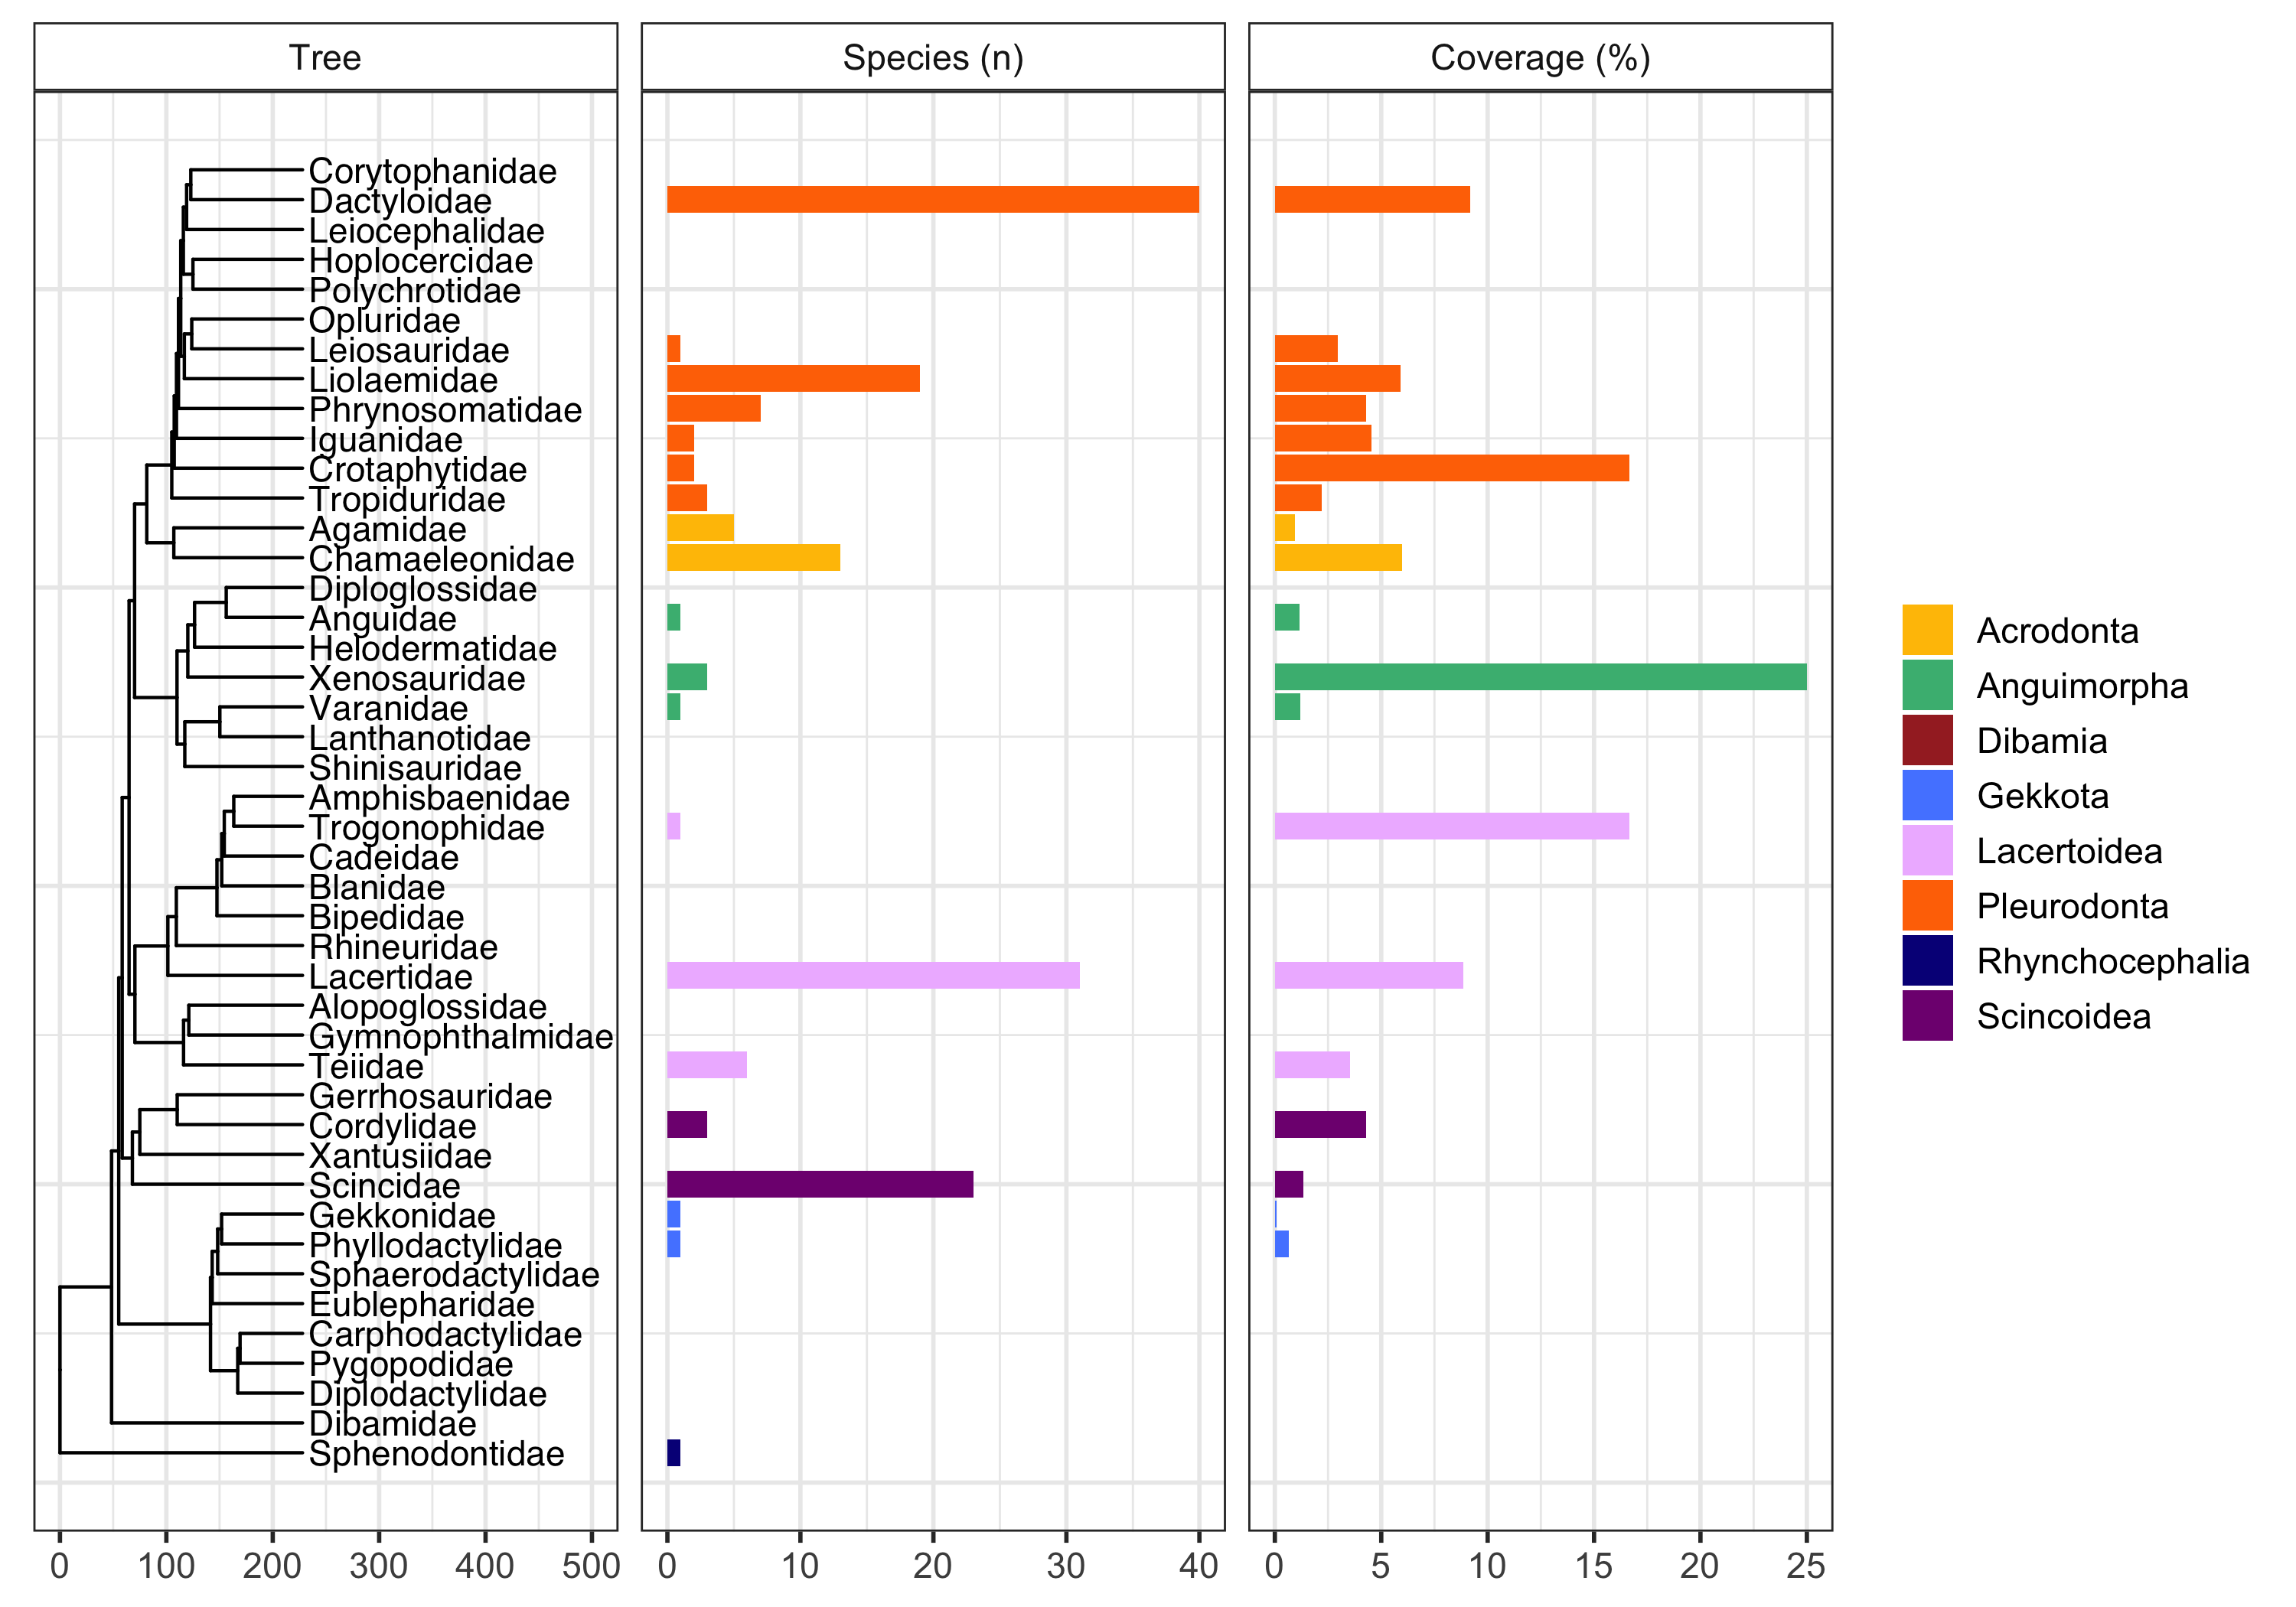
\includegraphics[width = \linewidth]{figures/phylogeny-data-coverage.png}
  \caption{Family-level coverage of the bite-force dataset (n = 164 species). 
  The left-hand panel shows the family level phylogeny, the central panel shows the number of species from each family in our dataset, and the right-hand panel shows the percentage of species from that family \citep[from][]{uetz2020reptile} that are in our dataset. 
  Sphenodontidae (Rhynchocephalia) contains only one species, \textit{Sphenodon punctatus}, and has 100\% coverage so was removed from the right-hand panel to prevent it from compressing the x-axis. 
  Colours indicate higher taxonomic groupings.
}
  \label{fig-data-coverage}
\end{figure}


% figure 2
\newpage
\begin{figure}[h]
 \centering
  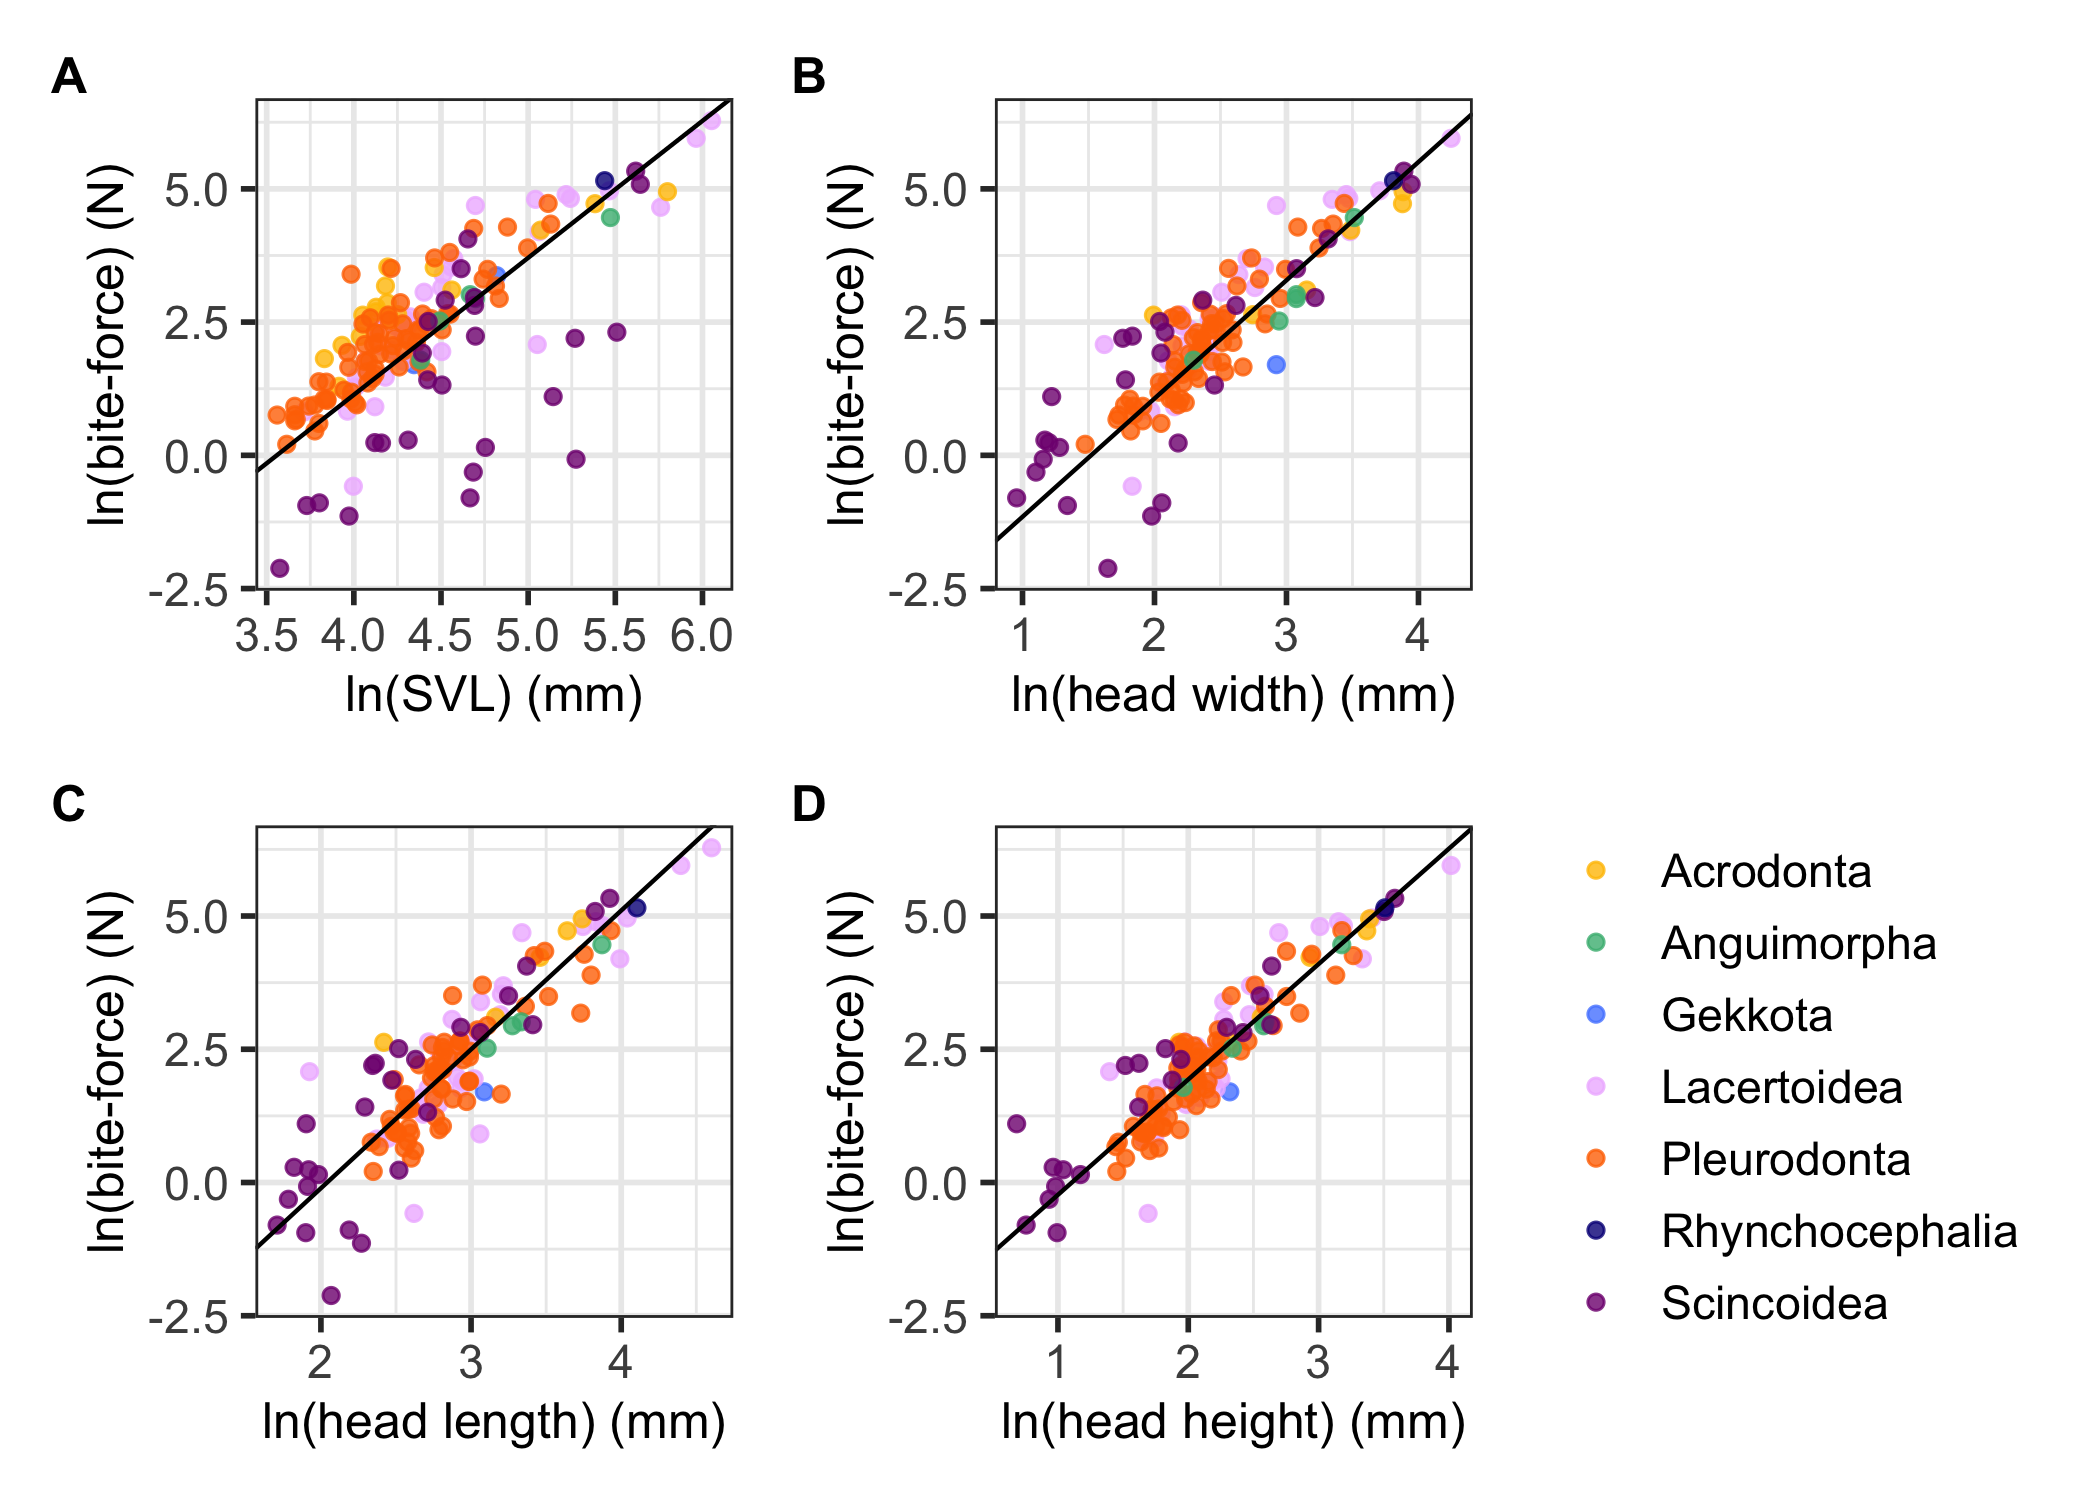
\includegraphics[width = \linewidth]{figures/bodysize-bite-force-coloured.png}
  \caption{The relationship between bite-force and each of the four body size measures for species from different higher taxonomic groupings. 
  (A) snout vent length (SVL; n = 161); (B) head width (n = 142); (C) head length (n = 136); and (D) head height (n = 136). 
  Points are slightly transparent to show where they overlap. 
  The lines are taken from phylogenetic generalised least squares (PGLS) models of bite-force as a function of body size (Table S5). 
  There were no significant differences among higher taxonomic groupings (Table 1). 
  }
  \label{fig-size-biteforce}
\end{figure}


% figure 3
\newpage
\begin{figure}[h]
 \centering
  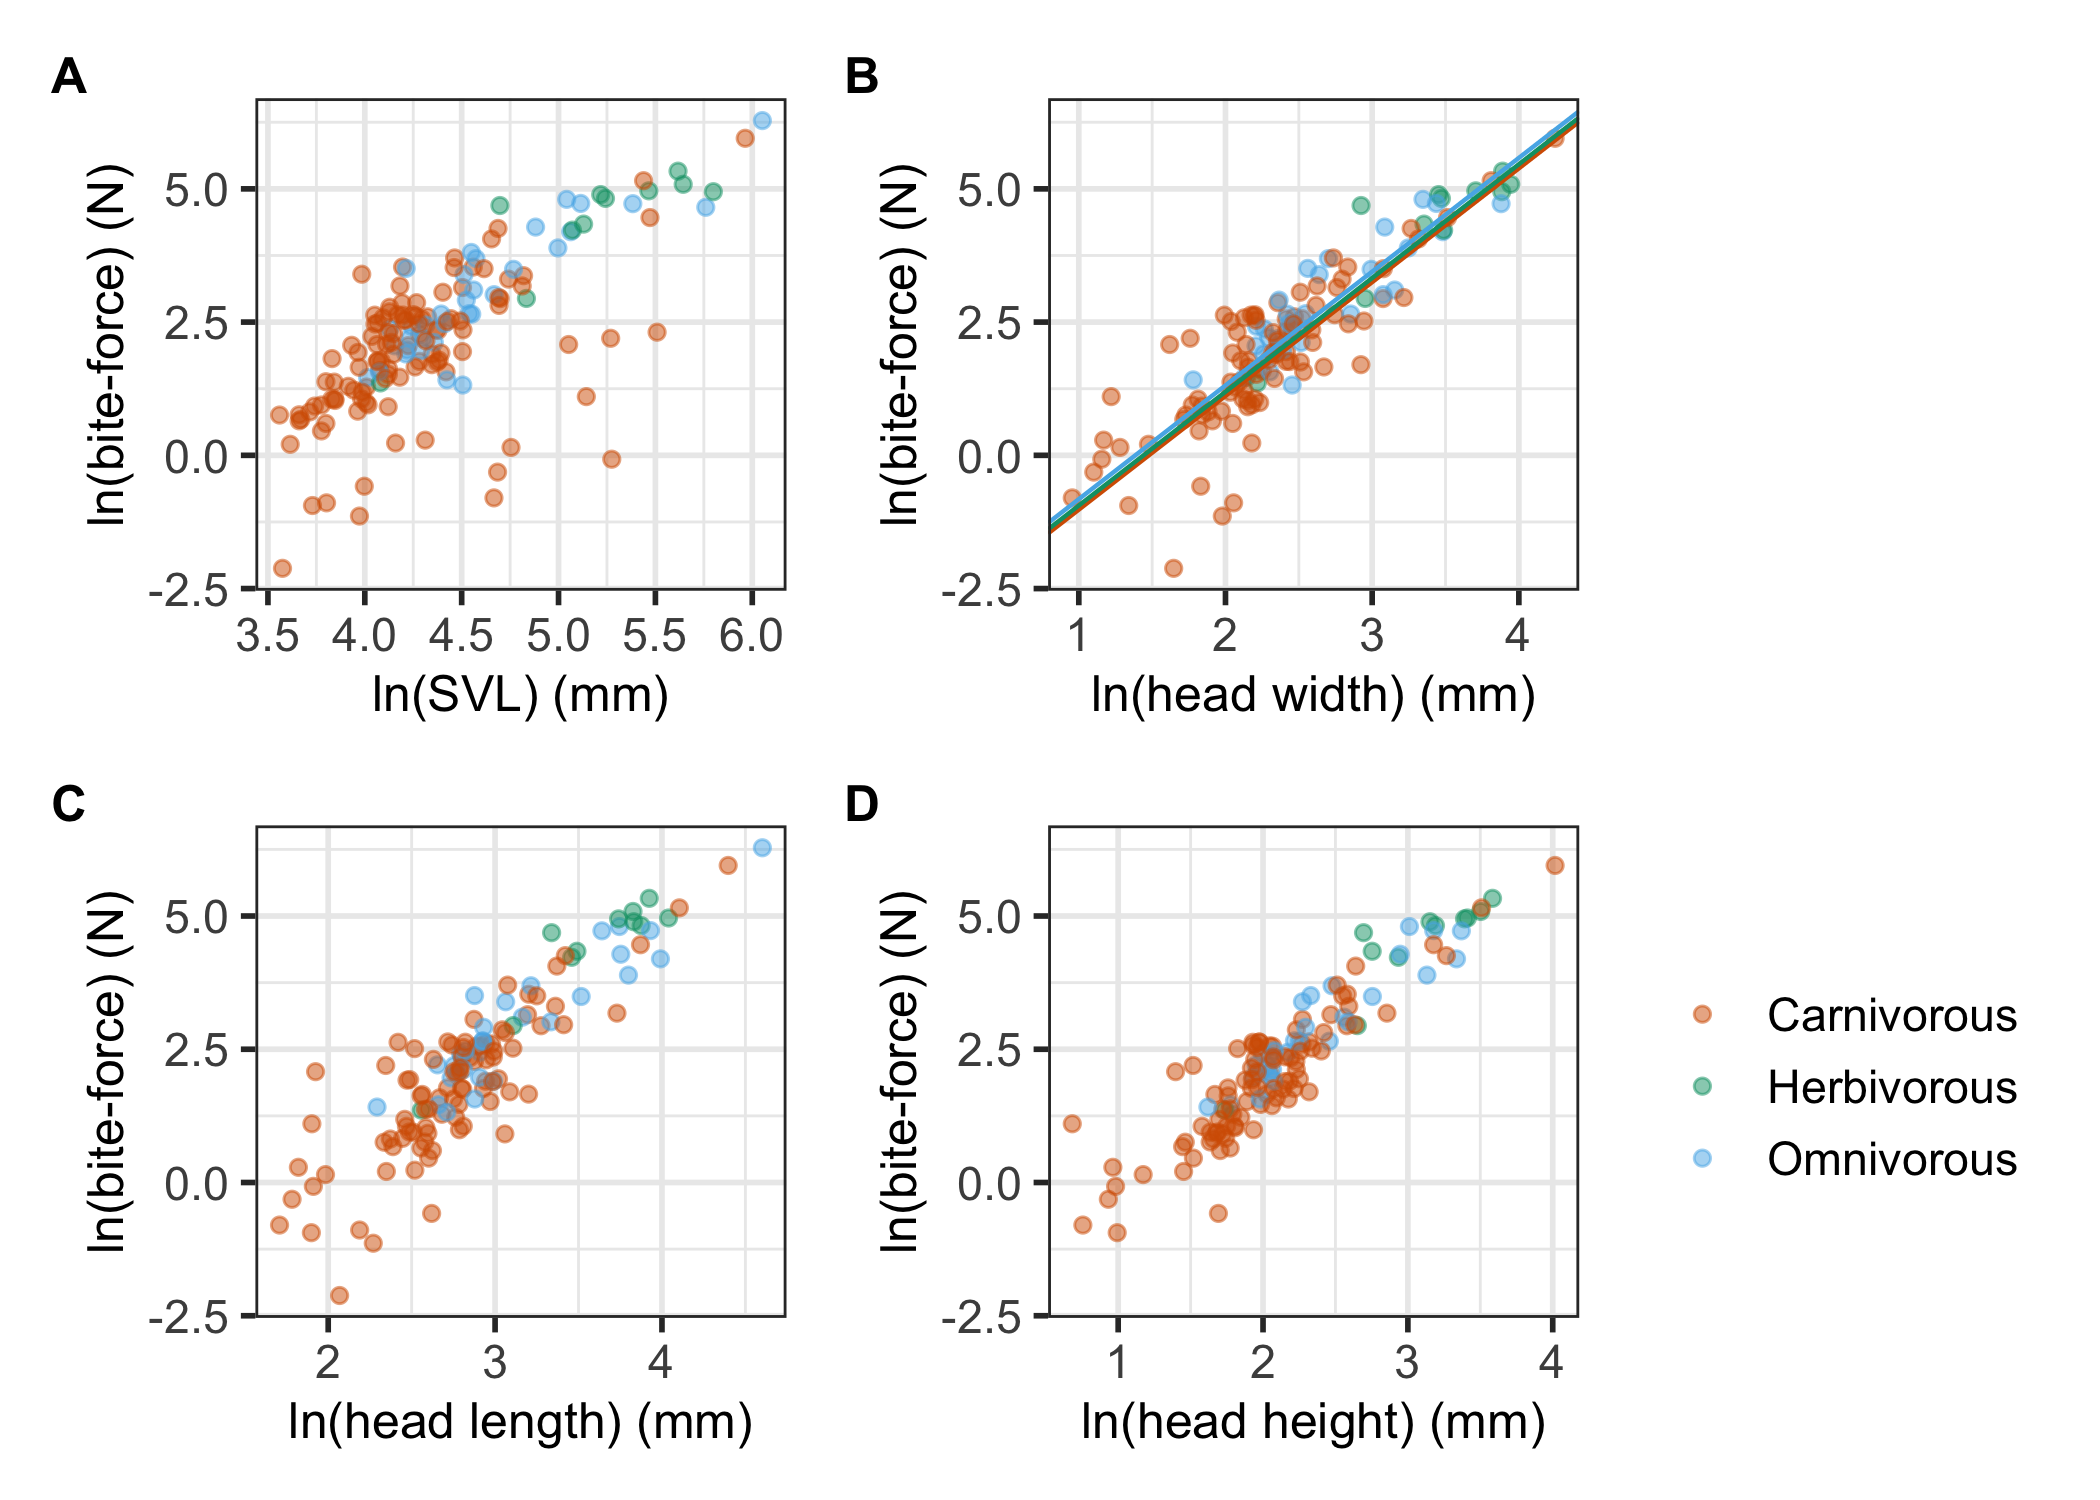
\includegraphics[width = \linewidth]{figures/bodysize-bite-force-diet.png}
  \caption{The relationship between bite-force and each of the four body size measures for species with different diets. 
  (A) snout vent length (SVL; n = 158); (B) head width (n = 139); (C) head length (n = 133); and (D) head height (n = 133). 
  Points are slightly transparent to show where they overlap. 
  The lines in (B) are taken from a phylogenetic generalised least squares (PGLS) model of bite-force as a function of head width and diet, where different diets have significantly different intercepts (Table 1). 
  There were no significant differences among diets for the other three body size measures (Table 1). 
}
  \label{fig-diet}
\end{figure}

% figure 4
\newpage
\begin{figure}[h]
 \centering
  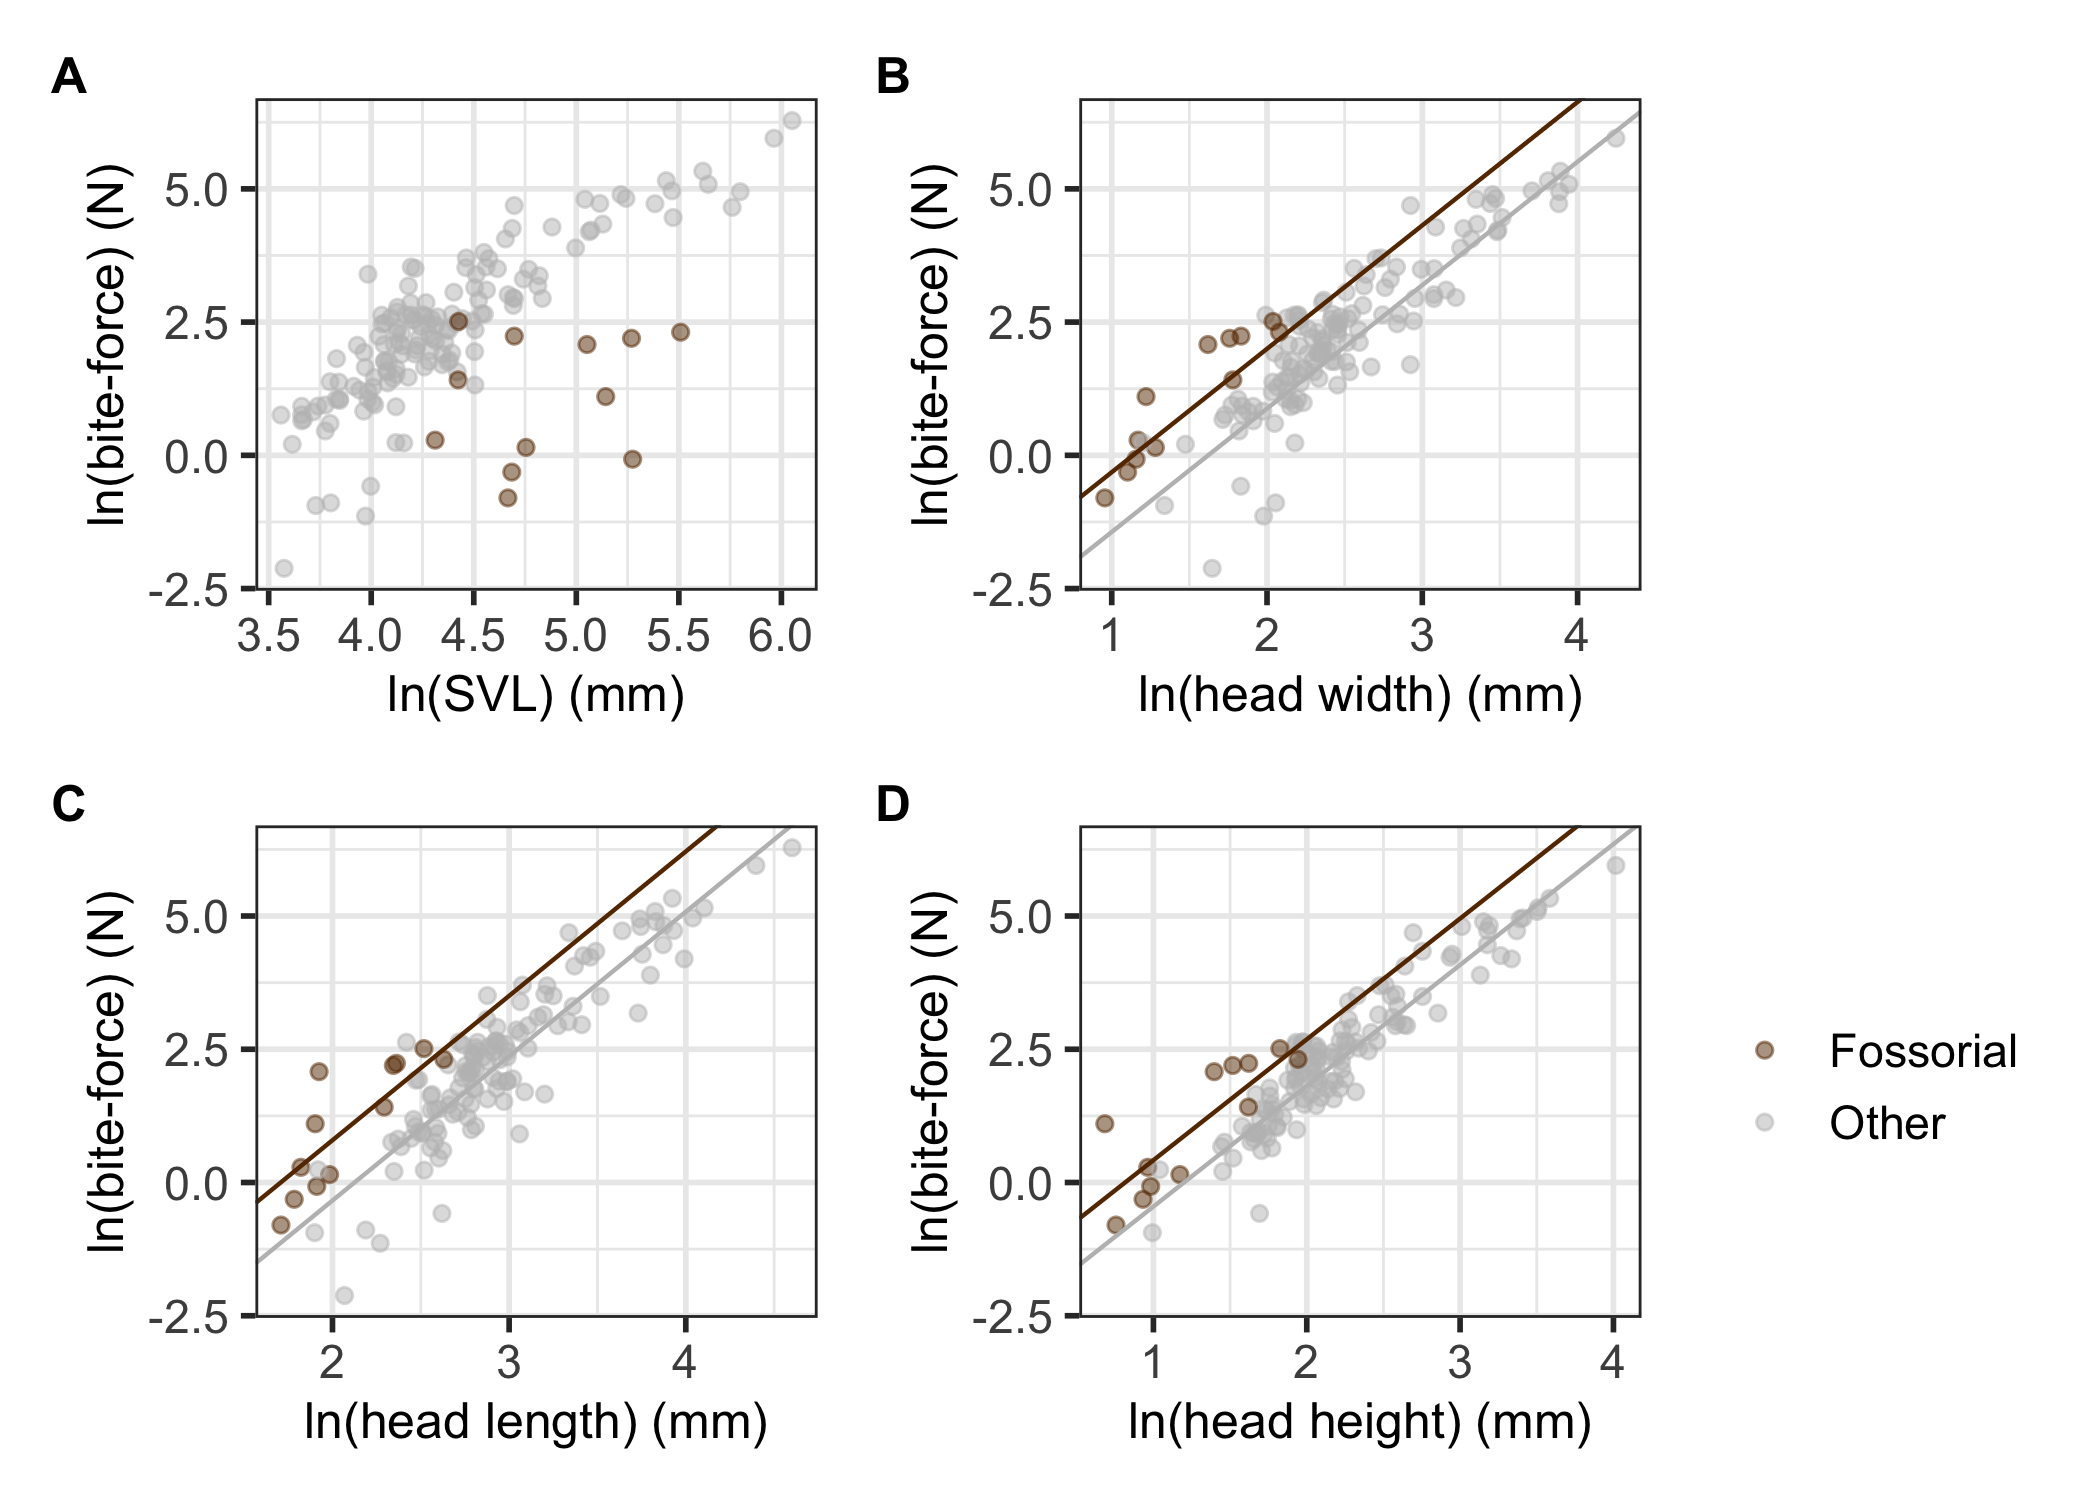
\includegraphics[width = \linewidth]{figures/bodysize-bite-force-fossorial.png}
  \caption{The relationship between bite-force and each of the four body size measures for species that are purely fossorial and those that are not. 
  (A) snout vent length (SVL; n = 161); (B) head width (n = 142); (C) head length (n = 136); and (D) head height (n = 136). 
  Points are slightly transparent to show where they overlap. 
  The lines in (B-D) are taken from phylogenetic generalised least squares (PGLS) models of bite-force as a function of body size and fossoriality, where fossorial and non-fossorial species have significantly different intercepts (Table 1). 
  There were no significant differences among fossorial and non-fossorial species for SVL (Table 1). 
}
  \label{fig-fossorial}
\end{figure}

%-------------------------------------------------------------------------------
% Tables
%-------------------------------------------------------------------------------
\newpage
\begin{landscape}
  % Table 1

\begin{longtable}{lccccccccccccccc}

\caption{Results from phylogenetic generalised least squares (PGLS) models of bite-force as a function of size, one of three covariates (tooth attachment type, diet, fossorial or not) and their interaction term. Size was snout vent length (SVL; mm), head width (HW; mm), head length (HL; mm), or head height (HH; mm). Significant p values are highlighted in bold. Bonferroni corrected p values (bonf p) are provided for all terms except the size term for which Bonferroni corrected p values were always $<$ 0.001. res df = residual degrees of freedom. df = degrees of freedom. $\lambda$ = Pagel's $\lambda$.}\\ 


% Header 1
\hline

\multicolumn{5}{c}{} &
\multicolumn{3}{c}{\textbf{size}} &
\multicolumn{4}{c}{\textbf{covariate}} &
\multicolumn{4}{c}{\textbf{interaction}}\\

  % Header 2
  \hline
  \textbf{covariate} &
  \textbf{size} &
  \textbf{res df} &
  \textbf{$\lambda$} &
  \textbf{r$^2$} &
  \textbf{df} &
  \textbf{F} &
  \textbf{p} &
  \textbf{df} &
  \textbf{F} &
  \textbf{p} &
  \textbf{bonf p} &
  \textbf{df} &
  \textbf{F} &
  \textbf{p} &
  \textbf{bonf p} \\

  % Body of table
\hline
tooth attachment & SVL & 157 & 0.946 & 0.723 & 1.000 & 416.8 & \textbf{$<$ 0.001} & 1.000 & 0.767 & 0.382 & 1.000 & 1.000 & 3.187 & 0.076 & 1.000 \\ 
tooth attachment & HW & 138 & 0.982 & 0.741 & 1.000 & 403.6 & \textbf{$<$ 0.001} & 1.000 & 0.053 & 0.818 & 1.000 & 1.000 & 3.049 & 0.083 & 1.000 \\ 
tooth attachment & HL & 132 & 0.96 & 0.709 & 1.000 & 330.1 & \textbf{$<$ 0.001} & 1.000 & 0.764 & 0.384 & 1.000 & 1.000 & 1.270 & 0.262 & 1.000 \\ 
tooth attachment & HH & 132 & 0.703 & 0.822 & 1.000 & 622.9 & \textbf{$<$ 0.001} & 1.000 & 0.344 & 0.558 & 1.000 & 1.000 & 1.230 & 0.269 & 1.000 \\ 
diet & SVL & 152 & 0.953 & 0.714 & 1.000 & 393.4 & \textbf{$<$ 0.001} & 2.000 & 0.706 & 0.495 & 1.000 & 2.000 & 1.008 & 0.367 & 1.000 \\ 
diet & HW & 133 & 1.000 & 0.806 & 1.000 & 546.8 & \textbf{$<$ 0.001} & 2.000 & 13.75 & \textbf{$<$ 0.001} & \textbf{$<$ 0.001} & 2.000 & 1.150 & 0.320 & 1.000 \\ 
diet & HL & 127 & 0.967 & 0.704 & 1.000 & 316.9 & \textbf{$<$ 0.001} & 2.000 & 1.026 & 0.362 & 1.000 & 2.000 & 0.328 & 0.721 & 1.000 \\ 
diet & HH & 127 & 0.681 & 0.822 & 1.000 & 613.5 & \textbf{$<$ 0.001} & 2.000 & 0.900 & 0.409 & 1.000 & 2.000 & 0.603 & 0.549 & 1.000 \\ 
fossorial & SVL & 157 & 0.949 & 0.741 & 1.000 & 445.3 & \textbf{$<$ 0.001} & 1.000 & 7.493 & \textbf{0.007} & 0.387 & 1.000 & 7.760 & \textbf{0.006} & 0.366 \\ 
fossorial & HW & 138 & 0.968 & 0.769 & 1.000 & 451.6 & \textbf{$<$ 0.001} & 1.000 & 16.48 & \textbf{$<$ 0.001} & \textbf{0.005} & 1.000 & 3.502 & 0.063 & 1.000 \\ 
fossorial & HL & 132 & 0.900 & 0.745 & 1.000 & 381.1 & \textbf{$<$ 0.001} & 1.000 & 14.89 & \textbf{$<$ 0.001} & \textbf{0.010} & 1.000 & 1.444 & 0.232 & 1.000 \\ 
fossorial & HH & 132 & 0.446 & 0.852 & 1.000 & 760.7 & \textbf{$<$ 0.001} & 1.000 & 16.53 & \textbf{$<$ 0.001} & \textbf{0.005} & 1.000 & 0.014 & 0.906 & 1.000 \\ 
\hline

\label{table_main_results}
\end{longtable}


\end{landscape}

%-------------------------------------------------------------------------------
% Table and figure legends
%-------------------------------------------------------------------------------

%\newpage
%\section{Table and figure legends}

%\textbf{Table 1}: Results from phylogenetic generalised least squares (PGLS) models of bite-force as a function of body size, one of six covariates and their interaction term. Body size was snout vent length (SVL; mm), head width (HW; mm), head length (HL; mm), or head height (HH; mm). Significant p values are highlighted in bold. Bonferroni corrected p values (bonf p) are provided for all terms except the body size term for which Bonferroni corrected p values were always $<$ 0.001. df = degrees of freedom. $\lambda$ = Pagel's $\lambda$.

\end{document}